\PassOptionsToPackage{backref=page}{hyperref}
\documentclass[aspectratio=169]{beamer}

% ========================== 导入必须的宏包 ==========================
\makeatletter
\def\input@path{{./style/}}
\makeatother
\usepackage{projectfonts}
% 每次使用时需要更新 style/titlepage.sty 里面的汇报文献信息
\usepackage{titlepage}
\usepackage{code}
\usepackage{UESTC}

% ========================== 根据需要导入其他宏包 ==========================
% 用于实现子图的宏包
% 不要使用{figure*},同时把\subfigure换成\subfloat
\usepackage{subcaption}
% 添加图片搜索路径
\graphicspath{{pictures/}}
% 绘图宏包
\usepackage{tikz}
\usepackage{pgfplots}
\pgfplotsset{compat=newest}
% 用于实现表格的宏包
\usepackage{booktabs}   % 支持表格符号
\usepackage{caption}    % 支持表格标题
\usepackage{multirow}   % 支持合并单元格
% 用于实现伪代码的宏包
\usepackage{algorithm}
\usepackage{algorithmic}
% 用于实现公式标注的内容
\usetikzlibrary{tikzmark}
\newcommand{\highlight}[2]{\textcolor{#1}{#2}}

% ========================== 处理警告信息 ==========================
\vfuzz=100pt % 忽略 overfull \vbox 的警告
\hfuzz=100pt % 忽略 overfull \hbox 的警告

\begin{document}
% ========================== 文档开始位置 ==========================

% 标题页
\begin{frame}
    \titlepage
\end{frame}

% 目录页
\begin{frame}{目录}
    \tableofcontents[sectionstyle=show]
\end{frame}

% ========================== 你的内容开始的地方 ==========================

\section{文字和列表}

\begin{frame}{列表}
    在slide中,比起段落文字,更建议使用列表。\\
    这是一个混合的列表:第一级使用有序列表,第二级使用无序列表。
    不建议超过两级列表。
    \begin{enumerate}
        \item 第一项
        \begin{itemize}
            \item 第一项的第一个子项,这是一个非常非常非常非常非常长的子项,用来展示换行的效果。
            \item 第一项的第二个子项
        \end{itemize}
        \item 第二项
        \begin{itemize}
            \item 第二项的第一个子项,这是一个较长的子项,用来展示效果。
            \item 第二项的第二个子项
        \end{itemize}
        \item 第三项,这是一个非常非常非常非常非常非常非常非常非常长的项,用来展示换行的效果。
    \end{enumerate}
\end{frame}

\begin{frame}{字号}
    \vspace{-1.8em}
    \begin{columns}[t]  % [t] 使内容顶部对齐
        % 左侧列
        \begin{column}{0.5\textwidth}
            \begin{itemize}
                \item {\tiny 这是 tiny 字号}
                \item {\scriptsize 这是 scriptsize 字号}
                \item {\footnotesize 这是 footnotesize 字号}
                \item {\small 这是 small 字号}
                \item {\normalsize 这是 normalsize 字号}
                \item {\large 这是 large 字号}
                \item {\Large 这是 Large 字号}
                \item {\LARGE 这是 LARGE 字号}
                \item {\huge 这是 huge 字号}
                \item {\Huge 这是 Huge 字号}
            \end{itemize}
        \end{column}
        % 右侧列
        \begin{column}{0.5\textwidth}
            \begin{itemize}
                \item {\wuhao 这是 五号字}
                \item {\dawuhao 这是 大五号字}
                \item {\xiaosi 这是 小四号字}
                \item {\banxiaosi 这是 半小四号字}
                \item {\sihao 这是 四号字}
                \item {\xiaosan 这是 小三号字}
                \item {\sanhao 这是 三号字}
                \item {\xiaoer 这是 小二号字}
                \item {\erhao 这是 二号字}
                \item {\yihao 这是 一号字}
            \end{itemize}
        \end{column}
    \end{columns}
\end{frame}

\begin{frame}{公式}
    Beamer中支持支持使用单个\$进行行内公式的书写,如 $E=mc^2$。\\
    Beamer中支持支持使用单个\$进行行内公式的书写,如 $E=mc^2$。\\
    \vspace{\baselineskip} % 空出一行的高度
    也支持使用\$\$进行行间公式的书写,如 
    $$
    E=mc^2
    $$
    并且还支持使用 \LaTeX{} 的数学环境来书写,且可以进行引用,如公式 \eqref{eq:1}。
    \begin{equation}
        \label{eq:1}
        E=mc^2
    \end{equation}
\end{frame}

\section{图片和表格}

\begin{frame}{图片1}
    \footnotesize
    在slide中,图片是一个重要的元素。此处重点展示图片的布局的两种方式:子图和分栏。\\
    子图将多个图片合并为一个图片。\\
    此时可以对子图进行引用,如图\ref{fig:subfig1};也可以对整个图片进行引用,如图\ref{fig:subfig}。
    \begin{figure}
        \centering
        \begin{subfigure}{0.3\textwidth}
            \centering
            
\includegraphics[width=\textwidth]{logo.pdf}
            \caption{校徽}
            \label{fig:subfig1}
        \end{subfigure}
        \begin{subfigure}{0.3\textwidth}
            \centering
            
\includegraphics[width=\textwidth]{logo.pdf}
            \caption{校徽}
            \label{fig:subfig2}
        \end{subfigure}
        \begin{subfigure}{0.3\textwidth}
            \centering
            
\includegraphics[width=\textwidth]{logo.pdf}
            \caption{校徽}
            \label{fig:subfig3}
        \end{subfigure}
        \vspace{-1em}
        \caption{电子科技大学校徽}
        \label{fig:subfig}
    \end{figure}
\end{frame}

\begin{frame}{图片2}
    分栏的方法更加灵活一点,因为可以轻易换成一侧图片一侧文字的布局。\\
    此时可以对每一侧的图片进行引用,如图\ref{fig:columnleft}和图\ref{fig:columnright}。
    \begin{columns}[t]  % [t] 使内容顶部对齐
        % 左侧列
        \begin{column}{0.5\textwidth}
            \begin{figure}
                \centering
                
\includegraphics[width=0.5\textwidth]{logo.pdf}
                \caption{电子科技大学校徽}
                \label{fig:columnleft}
            \end{figure}
        \end{column}
        % 右侧列
        \begin{column}{0.5\textwidth}
            \begin{figure}
                \centering
                
\includegraphics[width=0.5\textwidth]{logo.pdf}
                \caption{电子科技大学校徽}
                \label{fig:columnright}
            \end{figure}
        \end{column}
    \end{columns}
\end{frame}

\begin{frame}{图片3}
    这里展示一边图片一边文字的布局。\\
    \begin{columns}[t]  % [t] 使内容顶部对齐
        % 左侧列
        \begin{column}{0.5\textwidth}
            \begin{figure}
                \centering
                
\includegraphics[width=0.5\textwidth]{logo.pdf}
                \caption{电子科技大学校徽}
                \label{fig:columnfig}
            \end{figure}
        \end{column}
        % 右侧列
        \begin{column}{0.5\textwidth}
            \begin{itemize}
                \item 电子科技大学(University of Electronic Science and Technology of China)
                \item 是中华人民共和国教育部直属的全日制普通本科高校。
                \item 是“211工程”、“985工程优势学科创新平台”重点建设高校。
                \item logo如图\ref{fig:columnfig}所示。
            \end{itemize}
        \end{column}
    \end{columns}
\end{frame}

\begin{frame}{图片4}
    这里展示使用 tikz 来绘制插图。\\
    \begin{columns}[t]  % [t] 使内容顶部对齐
        % 左侧列
        \begin{column}{0.3\textwidth}
            \begin{figure}[!ht]
                \centering
                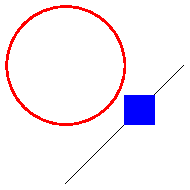
\includegraphics[width=0.4\textwidth]{tikz/pic1/pic.pdf}
                \caption{示例图片}
                \label{fig:pic1}
            \end{figure}
        \end{column}
        % 右侧列
        \begin{column}{0.7\textwidth}
            \begin{figure}[!ht]
                \centering
                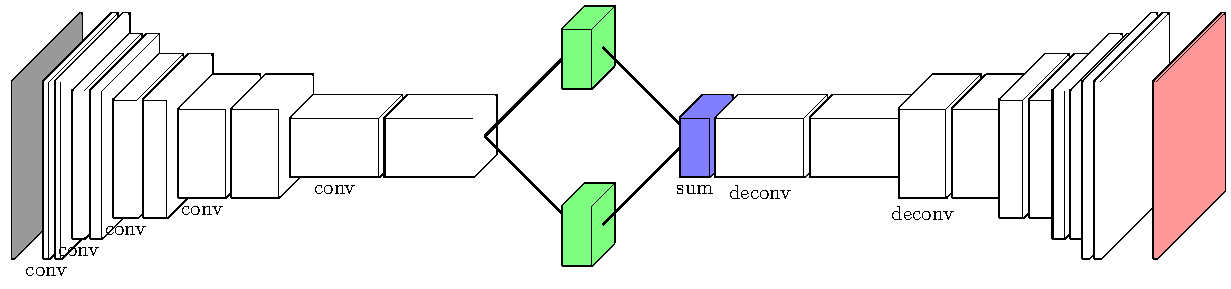
\includegraphics[width=\textwidth]{tikz/net/pic.pdf}
                \caption{示例图片}
                \label{fig:net}
            \end{figure}
        \end{column}
    \end{columns}
\end{frame}

\begin{frame}{表格}
    \begin{itemize}
        \item 表格是另一个重要的元素。此处展示一个简单的表格,如表\ref{tab:table}所示。
        \item 这个表格是直接从下载的论文tex原文\url{https://arxiv.org/abs/2312.15701}中复制而来,非常简单易用。
        \item 如果你有自己制作latex表格的需求,可以参考\href{https://www.tablesgenerator.com/}{Tables Generator}。
    \end{itemize}
    \vspace{-1em}
    \scriptsize
    \begin{table}
        \centering
        \begin{tabular}{lcccccccccc}
            \toprule
            \multirow{2}{*}{Method} & \multirow{2}{*}{Scale} & \multicolumn{2}{c}{Urban100} & \multicolumn{2}{c}{BSD100} & \multicolumn{2}{c}{Set14} & \multicolumn{2}{c}{Set5} & Standard \\
            \cmidrule(r){3-4} \cmidrule(r){5-6} \cmidrule(r){7-8} \cmidrule(r){9-10}
            & & PSNR & SSIM & PSNR & SSIM & PSNR & SSIM & PSNR & SSIM & Deviation\\ 
            \midrule
            KXNet & \multirow{4}{*}{x2} & 28.51 & 0.8667 & 30.38 & 0.8485 & 31.28 & 0.8697 & 35.00 & 0.9335 & \multirow{4}{*}{0} \\
            KXNet-$p4$ & & 28.91 & 0.8758 & 30.63 & 0.8564 & 31.64 & 0.8756 & 35.21 & 0.9362 &\\
            KXNet-$p8$ & & 28.49 & 0.8659 & 30.44 & 0.8505 & 31.45 & 0.8709 & 35.08 & 0.9344 &\\
            KXNet-$p8+$ & & 29.13 & 0.8808 & 30.73 & 0.8587 & 31.74 & 0.8772 & 35.35 & 0.9375 &\\
            \bottomrule
        \end{tabular}
        \caption{一个示例的表格}
        \label{tab:table}
    \end{table}
\end{frame}

\section{块}

\begin{frame}{块}
    \begin{block}{块的名称}
        \begin{itemize}
            \item A
            \item B
        \end{itemize}
    \end{block}	
\end{frame}
    
\begin{frame}{定义、定理、引理、证明}
    \begin{define}[定义名称]
        定义内容
    \end{define}
    \begin{lem}[引理名称]
        引理内容
    \end{lem}
    \begin{thm}[定理名称]
        定理内容(这里的定义、引理、定理分章节自动标号)
    \end{thm}
    \begin{proof}
        证明内容
    \end{proof}
\end{frame}

\begin{frame}{四分块的展示}
    \vspace{-1.8em}
    \tiny
    \begin{columns}[t]  % [t] 使内容顶部对齐
        % 左侧列
        \begin{column}{0.5\textwidth}
            \begin{block}{\scriptsize 第一个块的名称}
                测试第一个块
            \end{block}
            \begin{block}{\scriptsize 第二个块的名称}
                展示第二个块,包括列表和公式
                \begin{itemize}
                    \item 这是一个列表
                    \item 这是一个列表
                    \item 这是一个列表
                    \item 这是一个列表
                \end{itemize}
                下面是一个公式展示
                \begin{equation}
                    \label{eq:2}
                    E=mc^2
                \end{equation}
                进行较长的内容展示,以便更好的展示效果。
                这是一段很长很长很长很长很长很长很长很长很长很长很长很长很长很长很长很长很长很长很长很长很长很长很长很长很长很长很长很长的文字\\
                如果在块中公式太长了:\\
                $y=x_1+x_2+x3+x_4+x_5+x_6+x_7+x_8+x_9+x_{10}+x_{11}+x_{12}+x_{13}+x_{14}$
                \vspace{-1.5em}
                \begin{center}
                    \scalebox{0.7}{$y=x_1+x_2+x3+x_4+x_5+x_6+x_7+x_8+x_9+x_{10}+x_{11}+x_{12}+x_{13}+x_{14}$}
                \end{center}
            \end{block}
        \end{column}
        % 右侧列
        \begin{column}{0.5\textwidth}
            \begin{block}{\scriptsize 第三个块的名称}
                \begin{columns} % 可以选择不对齐,可能效果会更合适
                    % 左侧列
                    \begin{column}{0.4\textwidth}
                        \begin{itemize}
                            \item 这是一个列表
                            \item 这是一个列表
                            \item 这是一个列表
                            \item 这是一个列表
                        \end{itemize}
                    \end{column}
                    % 右侧列
                    \hspace{-3em}
                    \begin{column}{0.5\textwidth}
                        \vspace{-1.5em}
                        \begin{figure}
                            \centering
                            
\includegraphics[width=\textwidth]{logo.pdf}
                            % 在 block 中不是很适合添加标题
                            \label{fig:figinblock}
                        \end{figure}
                    \end{column}
                \end{columns}
            \end{block}	
            \begin{block}{\scriptsize 第四个块的名称}
                \begin{itemize}
                    \item 这是一个列表
                \end{itemize}
                \raggedright 
            \end{block}	
        \end{column}
    \end{columns}
\end{frame}

\section{代码}

\begin{frame}{介绍}
    \begin{enumerate}
        \item slide中并不是很适合展示大段代码,但是可以展示一些简短的代码片段。
        \item 这里的采用pandoc将md文件转换为beamer的方式来生成高量的代码。
        \item 相关的文件放在了code文件夹中,可以在其中查看。
        \begin{itemize}
            \item \texttt{code/convert\_to\_beamer.sh} 提供了转换的命令。
            \item \texttt{code/source.md} 提供了原始的Markdown代码。
            \item \texttt{code/source.tex} 提供了转换后的Beamer代码。
        \end{itemize}
        \item 以下是三种语言的代码片段展示。
        \item 为了更好的展示,建议使用分栏(三栏)的方式展示代码,以便控制背景的大小,不至于显得太空旷。
        \item 代码的字号建议为scriptsize或tiny。
    \end{enumerate}
\end{frame}

\begin{frame}[fragile]{python}
    \scriptsize
    \vspace{-2em}
    \begin{columns}[t]  % [t] 使内容顶部对齐
        \begin{column}{0.15\textwidth}
        \end{column}
        \begin{column}{0.7\textwidth}
            \begin{Shaded}
            \begin{Highlighting}[]
    \CommentTok{\# Import necessary libraries}
    \ImportTok{import}\NormalTok{ math}
    \ImportTok{import}\NormalTok{ os}

    \CommentTok{\# Function to calculate the square root}
    \KeywordTok{def}\NormalTok{ calculate\_sqrt(number):}
        \ControlFlowTok{return}\NormalTok{ math.sqrt(number)}

    \ControlFlowTok{if} \VariableTok{\_\_name\_\_} \OperatorTok{==} \StringTok{"\_\_main\_\_"}\NormalTok{:}
    \NormalTok{    number }\OperatorTok{=} \DecValTok{16}
    \NormalTok{    result }\OperatorTok{=}\NormalTok{ calculate\_sqrt(number)}
        \BuiltInTok{print}\NormalTok{(}\SpecialStringTok{f"The square root of }\SpecialCharTok{\{}\NormalTok{number}\SpecialCharTok{\}}\SpecialStringTok{ is }\SpecialCharTok{\{}\NormalTok{result}\SpecialCharTok{\}}\SpecialStringTok{"}\NormalTok{)}

        \CommentTok{\# Loop example}
        \ControlFlowTok{for}\NormalTok{ i }\KeywordTok{in} \BuiltInTok{range}\NormalTok{(}\DecValTok{5}\NormalTok{):}
            \BuiltInTok{print}\NormalTok{(}\SpecialStringTok{f"Loop index: }\SpecialCharTok{\{}\NormalTok{i}\SpecialCharTok{\}}\SpecialStringTok{"}\NormalTok{)}
            \end{Highlighting}
            \end{Shaded}
        \end{column}
        \begin{column}{0.15\textwidth}
        \end{column}
    \end{columns}
\end{frame}

\begin{frame}[fragile]{C}
    \tiny
    \vspace{-2em}
    \begin{columns}[t]  % [t] 使内容顶部对齐
        \begin{column}{0.2\textwidth}
        \end{column}
        \begin{column}{0.6\textwidth}
            \begin{Shaded}
    \begin{Highlighting}[]
    \PreprocessorTok{\#include }\ImportTok{\textless{}stdio.h\textgreater{}}
    \PreprocessorTok{\#include }\ImportTok{\textless{}stdlib.h\textgreater{}}
    \PreprocessorTok{\#include }\ImportTok{\textless{}string.h\textgreater{}}
    
    \CommentTok{// Function to add two numbers}
    \DataTypeTok{int}\NormalTok{ add}\OperatorTok{(}\DataTypeTok{int}\NormalTok{ a}\OperatorTok{,} \DataTypeTok{int}\NormalTok{ b}\OperatorTok{)} \OperatorTok{\{}
        \ControlFlowTok{return}\NormalTok{ a }\OperatorTok{+}\NormalTok{ b}\OperatorTok{;}
    \OperatorTok{\}}
    
    \DataTypeTok{int}\NormalTok{ main}\OperatorTok{()} \OperatorTok{\{}
        \DataTypeTok{int}\NormalTok{ x }\OperatorTok{=} \DecValTok{10}\OperatorTok{,}\NormalTok{ y }\OperatorTok{=} \DecValTok{20}\OperatorTok{,}\NormalTok{ result}\OperatorTok{;}
    \NormalTok{    result }\OperatorTok{=}\NormalTok{ add}\OperatorTok{(}\NormalTok{x}\OperatorTok{,}\NormalTok{ y}\OperatorTok{);}
    \NormalTok{    printf}\OperatorTok{(}\StringTok{"The result is: }\SpecialCharTok{\%d\textbackslash{}n}\StringTok{"}\OperatorTok{,}\NormalTok{ result}\OperatorTok{);}
    
        \CommentTok{// Loop example}
        \ControlFlowTok{for} \OperatorTok{(}\DataTypeTok{int}\NormalTok{ i }\OperatorTok{=} \DecValTok{0}\OperatorTok{;}\NormalTok{ i }\OperatorTok{\textless{}} \DecValTok{5}\OperatorTok{;}\NormalTok{ i}\OperatorTok{++)} \OperatorTok{\{}
    \NormalTok{        printf}\OperatorTok{(}\StringTok{"Loop index: }\SpecialCharTok{\%d\textbackslash{}n}\StringTok{"}\OperatorTok{,}\NormalTok{ i}\OperatorTok{);}
        \OperatorTok{\}}
    
        \ControlFlowTok{return} \DecValTok{0}\OperatorTok{;}
    \OperatorTok{\}}
    \end{Highlighting}
            \end{Shaded}
        \end{column}
        \begin{column}{0.2\textwidth}
        \end{column}
    \end{columns}
\end{frame}

\begin{frame}[fragile]{matlab}
    \scriptsize
    \vspace{-2em}
    \begin{columns}[t]  % [t] 使内容顶部对齐
        \begin{column}{0.1\textwidth}
        \end{column}
        \begin{column}{0.8\textwidth}
            \begin{Shaded}
    \begin{Highlighting}[]
    \CommentTok{\% Function to calculate the square root}
    \KeywordTok{function} \VariableTok{result} \OperatorTok{=} \VariableTok{calculate\_sqrt}\NormalTok{(}\VariableTok{number}\NormalTok{)}
        \VariableTok{result} \OperatorTok{=} \VariableTok{sqrt}\NormalTok{(}\VariableTok{number}\NormalTok{)}\OperatorTok{;}
    \KeywordTok{end}
    
    \CommentTok{\% Main script}
    \VariableTok{number} \OperatorTok{=} \FloatTok{16}\OperatorTok{;}
    \VariableTok{result} \OperatorTok{=} \VariableTok{calculate\_sqrt}\NormalTok{(}\VariableTok{number}\NormalTok{)}\OperatorTok{;}
    \VariableTok{fprintf}\NormalTok{(}\SpecialStringTok{\textquotesingle{}The square root of \%d is \%.2f\textbackslash{}n\textquotesingle{}}\OperatorTok{,} \VariableTok{number}\OperatorTok{,} \VariableTok{result}\NormalTok{)}\OperatorTok{;}
    
    \CommentTok{\% Loop example}
    \KeywordTok{for} \VariableTok{i} \OperatorTok{=} \FloatTok{1}\OperatorTok{:}\FloatTok{5}
        \VariableTok{fprintf}\NormalTok{(}\SpecialStringTok{\textquotesingle{}Loop index: \%d\textbackslash{}n\textquotesingle{}}\OperatorTok{,} \VariableTok{i}\NormalTok{)}\OperatorTok{;}
    \KeywordTok{end}
    \end{Highlighting}
            \end{Shaded}
        \end{column}
        \begin{column}{0.1\textwidth}
        \end{column}
    \end{columns}
\end{frame}

\begin{frame}{伪代码}
    \begin{algorithm}[H]
        \caption{冒泡排序算法}
        \begin{algorithmic}[1] % [1] 表示每行编号
            \REQUIRE 一个数组 $A$,包含 $n$ 个元素
            \ENSURE 数组 $A$ 被升序排序
            \FOR{$i = 1$ 到 $n-1$}
                \FOR{$j = 1$ 到 $n-i$}
                    \IF{$A[j] > A[j+1]$}
                        \STATE 交换 $A[j]$ 和 $A[j+1]$
                    \ENDIF
                \ENDFOR
            \ENDFOR
            \RETURN $A$
        \end{algorithmic}
    \end{algorithm}
\end{frame}

\section{引用与跳转}

\begin{frame}{文献引用}
    这一个页面展示了文献引用的效果。\\
    首先请将所需要引用的文献(格式为BibTeX)添加到bibliography.bib文件中。\\
    然后在文中使用\textbackslash cite\{key\}进行引用,此时会自动在文末生成引用列表。\\
    \begin{enumerate}
        \item 第一个文献引用\cite{fu2022kxnet}
        \item 第二个文献引用\cite{celledoni2021equivariant}
        \item 第三个文献引用\cite{chen2023imaging}
        \item 第四个文献引用\cite{sannai2021improved}
        \item 第五个文献引用\cite{fu2024rotation}
        \item 第六个文献引用\cite{xie2022fourier}
        \item 第七个文献引用\cite{weiler2018learning}
    \end{enumerate}
\end{frame}

\begin{frame}{其他引用}
    这个页面展示了包括公式、图片、表格的引用效果。\\
    与文献引用不同,没有办法直接跳转回到这个页面,但是可以借助跳转功能实现返回效果。
    \begin{enumerate}
        \item 公式引用:公式 \eqref{eq:1}
        \item 图片引用:图 \ref{fig:subfig1} 和图 \ref{fig:columnfig}
        \item 表格引用:表 \ref{tab:table}
    \end{enumerate}
\end{frame}

\begin{frame}[label=jump1]{跳转(第一页)}
    这是一个跳转的slide。\\
    点击\hyperlink{jump2}{这里}可以跳转到第二页。
\end{frame}

\begin{frame}[label=jump2]{跳转(第二页)}
    \vspace{2cm}
    这是一个跳转的slide。\\
    点击\hyperlink{jump1}{这里}可以跳转回第一页。\\
    跳转按钮可以改变颜色,且放置在任何位置,例如页面左下角。\\
    \vspace{2cm}
    \hyperlink{jump1}{\beamergotobutton{跳转}}
\end{frame}

\section{新增加的模版}

\begin{frame}{新的四分块}
    \begingroup  % 局部作用域
    
    % ========================== 本页专用设置 ==========================
    % 四分块意味着整个页面展示的内容比较多,因此可能需要对默认的字体进行更换(更换为更小的字体)
    % 因为无序列表和有序列表都是固定的字号,因此在这里对无序列表和有序列表进行了局部的重新定义
    % 图片的标号使用的字号也是在固定的,这里还没有进行重新定义,是一个 TODO 项目
    \def\fbtitlefont{\scriptsize}
    \def\fbfont{\tiny}

    \newenvironment{il}{%
    \begingroup
    \let\originalitemcommand\item
    \renewcommand{\item}{\originalitemcommand\fbfont}
    \setbeamertemplate{itemize item}{\fbfont$\bullet$}
    \setbeamertemplate{itemize subitem}{\fbfont$\bullet$}
    \begin{itemize}%
        \setlength{\itemsep}{0pt}%
        \setlength{\parskip}{0pt}%
        \setlength{\leftskip}{-1em}%
    }{%
    \end{itemize}
    \endgroup
    }
    \newenvironment{el}{%
    \begingroup
    \let\originalenumcommand\item
    \renewcommand{\item}{\originalenumcommand\fbfont}
    \begin{enumerate}%
        \setlength{\itemsep}{0pt}%
        \setlength{\parskip}{0pt}%
        \setlength{\leftskip}{-1em}%
    }{%
    \end{enumerate}
    \endgroup
    }

    % ========================== 四分块开始的地方 ==========================
    % 每一个minipage都是一个块,分为左上、左下、右上、右下
    \begin{columns}[t]
        \begin{column}{0.5\textwidth}
            % ========================== 左上开始 ==========================
            \begin{minipage}[t]{\linewidth}
                \fbtitlefont
                左上标题\par
                \vspace{-0.5em}
                \textcolor{uestc}{\rule{\linewidth}{0.5pt}}\par
                \vspace{0.5em}
                \fbfont % 左上正文开始的地方:
                测试第一个块
            \end{minipage}
            % ========================== 左上结束 ==========================
        
            \vspace{1em}

            % ========================== 左下开始 ==========================
            \begin{minipage}{\linewidth}
                \fbtitlefont
                左下标题\par
                \vspace{-0.5em}
                \textcolor{uestc}{\rule{\linewidth}{0.5pt}}\par
                \vspace{0.5em}
                \fbfont % 左下正文开始的地方:
                展示第二个块,主要测试列表:
                \begin{el}
                    \item 第一项
                    \begin{il}
                        \item 第一项的第一个子项,这是一个非常非常非常非常非常长的子项,用来展示换行的效果。
                        \item 第一项的第二个子项
                    \end{il}
                    \item 第二项
                    \begin{il}
                        \item 第二项的第一个子项,这是一个较长的子项,用来展示效果。
                        \item 第二项的第二个子项
                    \end{il}
                    \item 第三项,这是一个非常非常非常非常非常非常非常非常非常长的项,用来展示换行的效果。
                \end{el}
            \end{minipage}
            % ========================== 左下结束 ==========================
        \end{column}
        
        \begin{column}{0.5\textwidth}
            % ========================== 右上开始 ==========================
            \begin{minipage}[t]{\linewidth}
                \fbtitlefont
                右上标题\par
                \vspace{-0.5em}
                \textcolor{uestc}{\rule{\linewidth}{0.5pt}}\par
                \vspace{0.5em}
                \fbfont % 右上正文开始的地方:
                \begin{figure}
                    \centering
                    
\includegraphics[height=2cm]{logo.pdf}
                    % \caption{电子科技大学校徽}
                    \label{fig:four-block-fig}
                \end{figure}
            \end{minipage}
            % ========================== 右上结束 ==========================
        
            \vspace{1em}
        
            % ========================== 右下开始 ==========================
            \begin{minipage}{\linewidth}
                \fbtitlefont
                右下标题\par
                \vspace{-0.5em}
                \textcolor{uestc}{\rule{\linewidth}{0.5pt}}\par
                \vspace{0.5em}
                \fbfont % 右下正文开始的地方:
                上面的图片内容是电子科技大学的校徽,

                展示了一个图片的效果。
            \end{minipage}
            % ========================== 右下结束 ==========================
        \end{column}
    \end{columns}
    
    \endgroup
\end{frame}

\begin{frame}{新的公式展示方案}
    来源于:\texttt{https://github.com/synercys/annotated\_latex\_equations}
    
    现在已经可以在这上面使用了,使用方法如下:

    \par \vspace{4em}

    \tikzset{remember picture, overlay}

    \[
    \Pr[\tikzmarknode{x}{\mathcal{X}}(\cdot) \in \tikzmarknode{s}{\mathcal{S}}] \leq e^\epsilon \cdot \Pr[\mathcal{X}(\cdot) \in \mathcal{S}]
    \]

    \begin{tikzpicture}[overlay, remember picture, >=stealth, nodes={align=left, inner ysep=1pt}, <-]
        % 标注 x
        \path (x.north) ++ (-4em,2em)
        node[anchor=south, color=blue!67, align=left, xshift=2em] (x_label)
        {\scriptsize system \\ 
        \scriptsize state};
        \draw [color=blue!87] (x.north) |- ([xshift=-2em] x_label.south);

        % 标注 s
        \path (s.south) ++ (4em,-2em)
        node[anchor=north, color=red!67, align=left, xshift=-2em] (s_label)
        {\scriptsize $\mathcal{S} \subseteq \mathrm{Range}(\mathcal{X})$};
        \draw [color=red!87] (s.south) |- ([xshift=2em] s_label.north);
    \end{tikzpicture}
\end{frame}

\section{参考文献与致谢}

\begin{frame}[allowframebreaks]{引用}
    \tiny\bibliographystyle{unsrt}
    \bibliography{bibliography}
\end{frame}

\begin{frame}{结束语}
    \begin{center}
        {\Huge\calligra Thanks!}
    \end{center}
\end{frame}

\end{document}